% !Mode:: "TeX:UTF-8"
%%%%%%%%%%%%%%%%%%%%%%%%%%%%%%%%%%%%%%%%%%%%%%%%%%%%%%%%%%%%%%%%%%%%%%%%%%%%%%%%
%          ,
%      /\^/`\
%     | \/   |                CONGRATULATIONS!
%     | |    |             SPRING IS IN THE AIR!
%     \ \    /                                                _ _
%      '\\//'                                               _{ ' }_
%        ||                     hithesis v3                { `.!.` }
%        ||                                                ',_/Y\_,'
%        ||  ,                   dustincys                   {_,_}
%    |\  ||  |\          Email: yanshuoc@gmail.com             |
%    | | ||  | |            https://yanshuo.site             (\|  /)
%    | | || / /                                               \| //
%    \ \||/ /       https://github.com/dustincys/hithesis      |//
%      `\\//`   \\   \./    \\ /     //    \\./   \\   //   \\ |/ /
%     ^^^^^^^^^^^^^^^^^^^^^^^^^^^^^^^^^^^^^^^^^^^^^^^^^^^^^^^^^^^^^^
%%%%%%%%%%%%%%%%%%%%%%%%%%%%%%%%%%%%%%%%%%%%%%%%%%%%%%%%%%%%%%%%%%%%%%%%%%%%%%%%
\documentclass[fontset=fandol,toc=true,type=master,stage=opening,campus=harbin]{hithesisart}
% 此处选项中不要有空格
%%%%%%%%%%%%%%%%%%%%%%%%%%%%%%%%%%%%%%%%%%%%%%%%%%%%%%%%%%%%%%%%%%%%%%%%%%%%%%%%
% 必填选项
% type=doctor|master|bachelor
% stage=opening|midterm
%%%%%%%%%%%%%%%%%%%%%%%%%%%%%%%%%%%%%%%%%%%%%%%%%%%%%%%%%%%%%%%%%%%%%%%%%%%%%%%%
% 选填选项（选填选项的缺省值已经尽可能满足了大多数需求，除非明确知道自己有什么
% 需求）
% campus=shenzhen|weihai|harbin
%   含义：校区选项，默认harbin
% fontset=windows|mac|ubuntu|fandol
%   含义：前三个对应各自系统，fandol是开源字体。
% toc=true|false
%   含义：是否显示目录，默认true
% newtxmath=true|false
%    含义：是否使用 times 风格数学字体，默认true
% print=true|false
%   含义：是否在封面后增加一个空白页用于打印，默认false
% bibauthorupper=full|preserve
%   含义：参考文献列表中作者名是否转为全大写，full表示全大写，preserve
%   表示维持.bib中的大小写。默认preserve。注意本选项只管大小写，并且
%   只在使用\bibliographystyle{hithesis}或者{hitszthesis}时生效。
% bibmaxauthor=<自然数>
%   含义：参考文献列表中每条文献显示的最大作者数量，如有更多作者会自动添加
%   "et al."或“等”（如果本条文献language={zh}或"zh"）。 0为全部显示。默认3.
%   该选项只在使用\bibliographystyle{hithesis}或者{hitszthesis}时生效。
% biblabelalign=left|right
%   含义：参考文献列表中的标号是左对齐(left)还是右对齐(right)。默认right.
%   在加入此选项前是左对齐，但这使文献达到100篇时第1-9篇文献标号后空格过大。
%%%%%%%%%%%%%%%%%%%%%%%%%%%%%%%%%%%%%%%%%%%%%%%%%%%%%%%%%%%%%%%%%%%%%%%%%%%%%%%%


\graphicspath{{figures/}}

%%%%%%%%%%%%%%%%%%%%%%%%%%%%%%%%%%%%%%%%%%%%%%%%%%%%%%%%%%%%%%%%%%%%%%%%%%%%%%%%
% 三级标题（subsubsection，如 4.1.1 研究内容一）的上下间距
%   模板默认仅 3bp（hithesisart.cls 第 357-365 行），配合小四字号后，
%   标题与下文之间的行距（约 13.5pt）明显小于正文行距（20.4pt），观感偏挤。
%   此处与二级标题对齐：上方 7bp 留白，下方 6bp（略小于二级以保持层级）。
%   如需恢复模板默认，删除下面这个 \ctexset 块即可。
%%%%%%%%%%%%%%%%%%%%%%%%%%%%%%%%%%%%%%%%%%%%%%%%%%%%%%%%%%%%%%%%%%%%%%%%%%%%%%%%
\ctexset{
  subsubsection={
    beforeskip=7bp,
    afterskip=6bp,
  }
}

\begin{document}

% !Mode:: "TeX:UTF-8"

\hitsetup{
  %******************************
  % 注意：
  %   1. 配置里面不要出现空行
  %   2. 不需要的配置信息可以删除
  %******************************
  ctitlecover={面向企业知识库的知识冲突消解与持续演化关键技术研究},%放在封面中使用，自由断行
  ctype={学位论文},%学位论文/实践成果
  caffil={计算学部},
  csubject={计算机科学与技术},
  cauthor={郑小博},
  cstudentid={25S003004},
  csupervisor={刘宏伟},
  % 日期自动使用当前时间，若需指定按如下方式修改：
  %cdate={盘古开天地}
  % cenrolldate={公元2020年}
}

\makecover

% 深圳校区硕士开题报告结构 ------------------------------------------

% !Mode:: "TeX:UTF-8"
%%%%%%%%%%%%%%%%%%%%%%%%%%%%%%%%%%%%%%%%%%%%%%%%%%%%%%%%%%%%%%%%%%%%%%%%%%%%%%%
%                          _
%  _____ ____ _ _ __  _ __| |___ ___
% / -_) \ / _` | '_ \ / -_|_-<
% \___/_\_\__,_|_|_|_| .__/_\___/__/
%                    |_|
%  _              _         _   _
% | |__ _  _   __| |_  _ __| |_(_)_ _  __ _  _ ___
% | '_ \ || | / _` | || (_-<  _| | ' \/ _| || (_-<
% |_.__/\_, | \__,_|\_,_/__/\__|_|_||_\__|\_, /__/
%       |__/                              |__/
%%%%%%%%%%%%%%%%%%%%%%%%%%%%%%%%%%%%%%%%%%%%%%%%%%%%%%%%%%%%%%%%%%%%%%%%%%%%%%%
% 硕士学位论文开题报告（深圳校区）
% 基于《开题报告-初稿.md》整理；插图绘制要点与生成提示词见 figures/ 目录。
% 修订记录：补课题来源；增补 WikiContradict/Mem0/真值发现/Lost-in-the-Middle
% 相关工作；统一冲突分类术语；表格列型 p{}；文风修订（压缩排比与模板句、
% 删除防御性表述）；6 处图位全部接入（5 张 AI 插图 + 4 幅系统截图子图）。
%%%%%%%%%%%%%%%%%%%%%%%%%%%%%%%%%%%%%%%%%%%%%%%%%%%%%%%%%%%%%%%%%%%%%%%%%%%%%%%
\section{课题来源及研究的目的和意义}

% TODO：若实际为导师纵向课题/企业横向课题，请替换为课题名称与编号
本课题基于导师在企业知识与检索增强生成方向的研究积累，以及 WeKnora 开源社区在企业知识库落地过程中暴露的真实需求提出。

\subsection{研究背景}

随着大语言模型（Large Language Model, LLM）能力的快速提升 \cite{che2023}，检索增强生成（Retrieval-Augmented Generation, RAG）已成为企业知识管理的主流技术范式：企业将内部文档构建为知识库，通过"检索—增强—生成"管线实现私有领域知识的准确问答与推理。以本课题所依托的 WeKnora 开源框架为例，其已支撑文档解析、混合检索、ReAct Agent 多步推理 \cite{yao2023}、自动 Wiki 蒸馏等完整能力链，覆盖了企业知识管理的核心场景，其中混合检索囊括 BM25 稀疏召回 \cite{robertson2009}、Dense 稠密召回与 GraphRAG 图谱增强等不同召回方式。

然而，当前 RAG 研究与工程实践普遍建立在\textbf{静态语料假设}之上，默认知识库内容准确、一致、不变，注意力集中在召回与生成的质量上。真实企业环境中，这一假设难以成立：

（1）知识冲突普遍存在。企业知识库不断收录各部门、各时期的新旧文档，文档之间存在大量事实性矛盾：政策口径调整后旧规定未同步（如退货政策由 7 天调整为 15 天）、同一产品参数在不同手册中记载冲突、文档过时但未被替换等。已有研究与系统观察表明，当检索命中互相矛盾的证据时，现有 RAG 系统往往盲从其中一方，或生成貌似折中的"调和式"回答，带来难以察觉的幻觉 \cite{liu2025halluc}。

（2）知识随对话流失。用户在与知识库的交互中会自然地提供增量信息，包括对既有知识的补充、更正以及本地化事实，例如"我们公司实际部署的是混合检索方案"。现有系统将对话视为一次性消费，增量知识随会话结束而流失，知识库无法从使用过程中演化。已有的 LLM 记忆研究多面向 Agent 私有记忆，缺少面向组织级知识资产的沉淀机制及其风险控制。

（3）知识资产缺乏来自使用过程的反馈信号。哪些文档被反复引用、哪些从未被使用、哪些内容处于未裁决的争议状态，这些信号对知识库的质量治理与检索排序均有价值，但在现有系统中普遍缺失。

\subsection{问题提出}

企业知识库要从静态资料库真正成长为可演化的知识资产，就必须回答本课题的核心科学问题：\textbf{在知识库内容非一致且持续演化的前提下，如何保障检索增强生成的可信性？}这一问题可拆解为三个方法子问题与一个系统支撑问题：

\begin{enumerate}
  \item \textbf{问题一（冲突检测与消解）}：如何在成本可控的前提下，检测大规模语料中跨文档的事实矛盾，区分事实矛盾、版本更新、互补共存等关系，并通过人机协同裁决维护存量语料的一致性？
  \item \textbf{问题二（冲突感知生成）}：当检索证据内部存在矛盾时，大模型的生成行为如何？如何设计冲突感知的检索与生成策略，使系统忠实呈现分歧而非盲目站队？
  \item \textbf{问题三（知识持续演化）}：如何从用户对话中识别值得入库的增量知识，决定是否写入、写到何处、如何写入，在知识沉淀收益与噪声污染风险之间取得可量化的平衡？
  \item \textbf{系统支撑}：上述能力所需的引用信号观测与层次化治理等基础，如何在真实系统上端到端落地并验证？
\end{enumerate}

\subsection{研究的目的及意义}

\textbf{理论意义}：
\begin{enumerate}
  \item 将多文档间的事实冲突检测形式化为语料级冲突对发现问题，补上现有研究偏重参数知识与检索证据冲突所留下的空白；
  \item 提出知识写入决策问题及其评测协议，刻画知识沉淀与污染之间的权衡，为 LLM 记忆与知识库演化研究补充新的问题定义；
  \item 刻画大模型在检索证据互相矛盾时的生成行为，深化对 RAG 忠实性的理解。
\end{enumerate}

\textbf{应用价值}：研究成果可直接落地于企业知识管理系统，解决知识库一致性维护、对话知识沉淀、知识资产治理等实际痛点。本课题依托的开源框架与原型系统为成果转化提供了现成载体。

\section{国内外在该方向的研究现状及分析}

\subsection{检索增强生成与知识库组织}

RAG 自 Lewis 等人提出以来已成为 LLM 知识外置的主流方案 \cite{lewis2020}。围绕检索质量与生成可信性，近年涌现大量改进：Self-RAG 通过反思令牌实现按需检索与自我批判 \cite{asai2024}；CRAG 引入检索质量评估与纠错机制 \cite{yan2024}；GraphRAG 利用实体图谱增强全局性问答 \cite{edge2024}；RAPTOR 构建递归摘要树以支持跨粒度检索 \cite{sarthi2024}；HippoRAG 借鉴海马体记忆索引理论设计个性化 PageRank 检索 \cite{gutierrez2024}。国内学界对 RAG 的评测体系、中文场景适配亦有系统性综述 \cite{gao2023,yuan2026}。

在企业知识组织方面，层次化摘要索引如 RAPTOR、GraphRAG 社区摘要多依赖自动聚类生成索引结构，对人类既有的目录、文件夹、产品线等组织语义利用不足，且普遍缺乏索引的\textbf{增量维护}与\textbf{使用信号反馈}机制。

现有 RAG 研究大多把知识库当作静态、一致的外部记忆，聚焦给定语料如何检索生成；语料本身的质量如何维护、如何演化，则很少进入研究视野。

\subsection{知识冲突研究}

知识冲突研究可分为四条线：

\textbf{（1）参数知识与检索证据的冲突。}Longpre 等人较早研究实体知识冲突对问答的影响 \cite{longpre2021}；Mallen 等人分析模型何时应信任参数知识 \cite{mallen2023}；Xu 等人（EMNLP 2023）刻画了 LLM 在参数知识与检索证据冲突时的"盲从"与"固执"行为 \cite{xu2023}；ConflictQA 进一步构建了该方向的评测基准 \cite{xie2024}。此类工作冲突的双方是"模型内部知识"与"外部证据"。

\textbf{（2）知识时效。}FreshLLMs / FreshQA 针对世界知识过时问题评测搜索增强能力 \cite{vu2024}，但其关注"证据新于参数"，而非语料内部的矛盾。

\textbf{（3）语料内部矛盾。}维基百科矛盾句检测、多文档摘要中的事实一致性校验等工作，如 Fool Me Twice 基准 \cite{zhong2021}，仍局限于句子级分类或摘要忠实性；生成端方面，WikiContradict 基准基于维基百科编辑标注的真实矛盾构建了 253 个人工标注样本，系统评测了主流 LLM 在双矛盾证据下的回答行为，发现模型普遍难以完整呈现分歧 \cite{hou2024wikicontradict}，但其语料限于维基百科、定位为生成端评测，未涉及冲突的\textbf{检测与消解管线}，也缺少企业场景中密集的版本更替类别。

\textbf{（4）多源真值发现（Truth Discovery）。}数据库与数据挖掘领域较早关注"多源冲突信息中判定何者为真"的问题 \cite{yin2008}，后续发展出考虑源可信度的系统性方法与综述 \cite{li2015}。该方向假设观测可结构化为"源—对象—取值"三元组，与本课题面向非结构化自然语言文档、需语义级比对的设定不同，但其源可信度估计思想对冲突裁决具有借鉴意义。

总体来看，参数与证据冲突的研究最为集中 \cite{xu2024survey}；语料内部冲突刚刚起步，除 WikiContradict 外尚无面向企业场景的\textbf{检测端}基准，也缺少覆盖检测、裁决、检索降权与生成呈现的端到端方法。

\subsection{LLM 记忆与知识库演化}

MemGPT 将操作系统的分页思想引入 LLM 记忆管理 \cite{packer2023}；MemoryBank 引入遗忘机制；A-MEM 提出 Agentic Memory 实现记忆的动态组织 \cite{xu2025amem}；Mem0 将记忆写入建模为 LLM 对 ADD / UPDATE / DELETE / NOOP 四种操作的决策，在个体记忆场景取得了成本与延迟优势 \cite{chhablani2025}，但允许覆盖式更新，不满足组织级资产的审计与回滚要求；Generative Agents 中的记忆流支持反思与检索 \cite{park2023}。自演化（self-evolving）方向的综述总结了 LLM 从经验中自我改进的各类范式 \cite{tao2024}。知识编辑方法，如 ROME、MEMIT 等，研究参数级知识的定位与修改 \cite{meng2022}，与本课题的语料级更新互补。

总体而言，现有记忆研究面向\textbf{Agent 个体记忆}，关注如何记住和召回交互历史；本课题面向\textbf{组织级知识资产}，关注如何把交互中有价值的事实沉淀为组织知识，并保证写入可审计、可回滚。对话驱动的知识库演化目前尚缺少对应的方法与评测基准。

\subsection{现状总结}

\begin{table}[htbp]
  \centering
  \caption{研究现状与缺口总结}
  \begin{tabular}{p{0.14\textwidth}p{0.40\textwidth}p{0.40\textwidth}}
    \toprule
    研究维度 & 现有工作 & 缺口 \\
    \midrule
    知识冲突 & 参数 vs.\ 证据冲突为主；真值发现处理结构化多源数据 & 非结构化企业语料的语料级冲突检测与消解缺基准、缺端到端方法 \\
    冲突下生成 & 参数—证据冲突下的行为刻画；WikiContradict 开始关注维基百科语料内矛盾 & 企业场景下、与检测/裁决联动的冲突感知检索与生成策略未系统研究 \\
    知识演化 & Agent 私有记忆（MemGPT、Mem0 等） & 组织级知识写入决策与污染控制缺评测方案 \\
    系统研究 & 原型/notebook 级实验 & 缺少真实系统支撑的端到端验证 \\
    \bottomrule
  \end{tabular}
\end{table}

% 图 1：研究定位四象限图（AI 生成；重制提示词见 figures/图片生成提示词.md）
\begin{figure}[htbp]
  \centering
  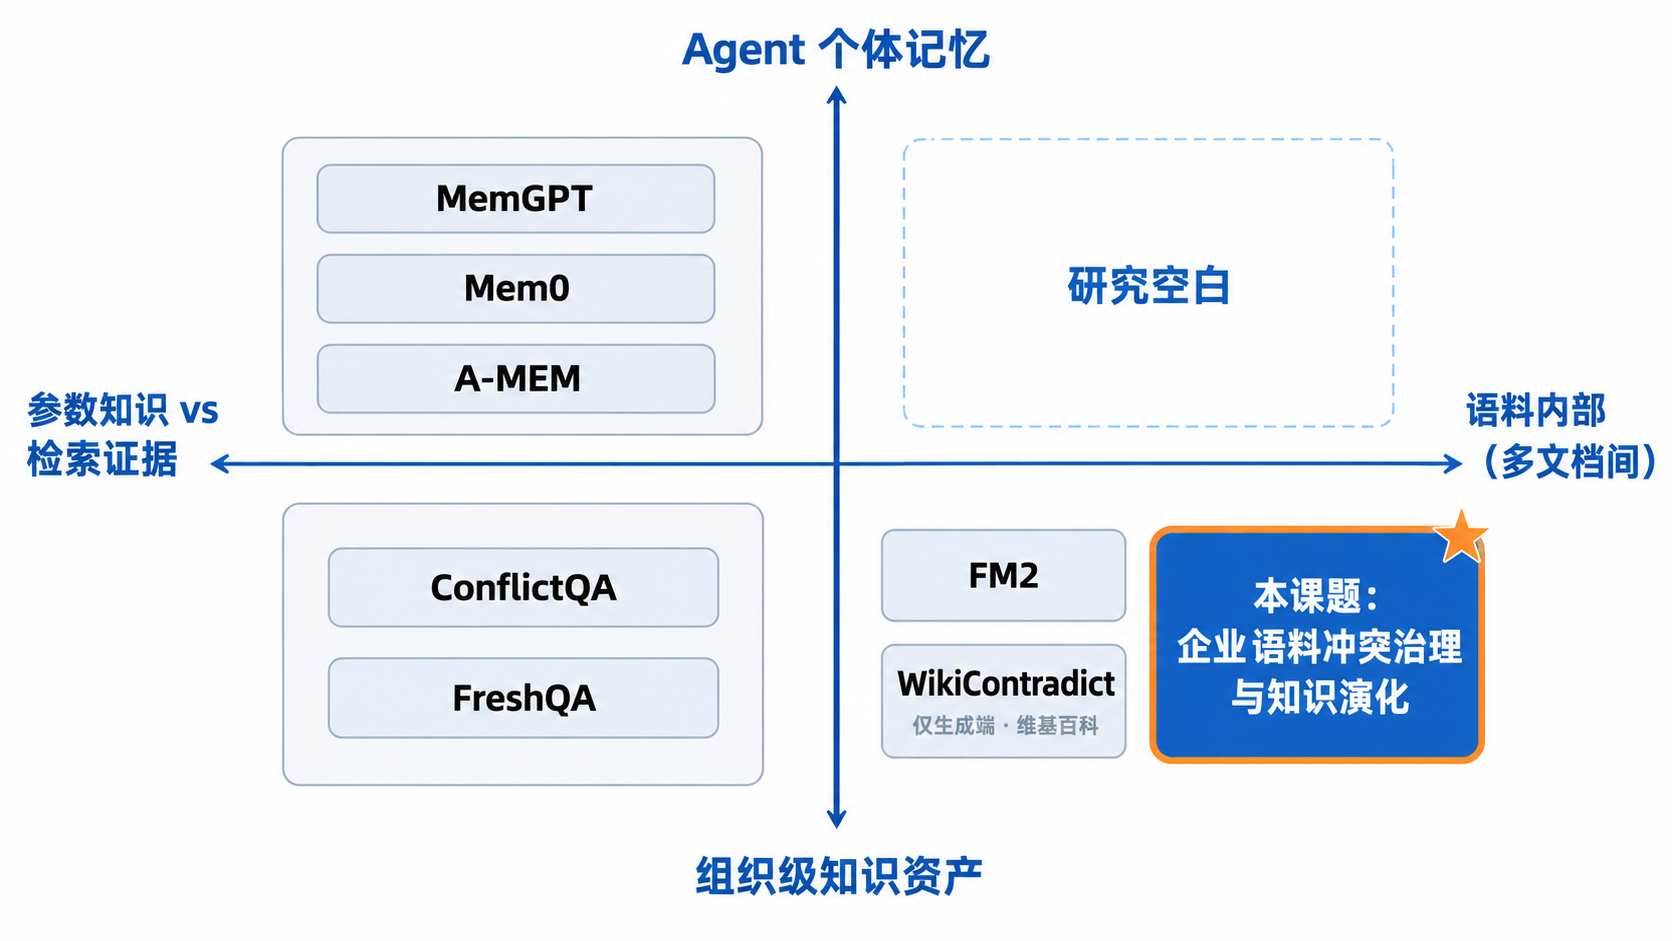
\includegraphics[width=0.85\textwidth]{gap-position}
  \caption{知识冲突与记忆研究方向定位}
  \label{fig:gap}
\end{figure}

本课题即针对图~\ref{fig:gap} 右下方的空白——非结构化企业语料的语料级冲突治理与组织级知识演化——展开。

\section{前期的理论研究与试验论证工作的结果}

依托 WeKnora 开源框架（Go 后端 + Vue 前端 + PostgreSQL/pgvector + asynq 异步任务队列 + Langfuse 全链路追踪 \cite{langfuse}），前期已完成四项原型工作，作为本课题的可行性基础，如表~\ref{tab:prework} 与图~\ref{fig:prototype} 所示。

% 图 2：前期原型系统截图组（4 幅子图：conflict-queue / ref-count / folder-manage / wiki-report）
\begin{figure}[htbp]
  \centering
  \subfigure[冲突裁决队列]{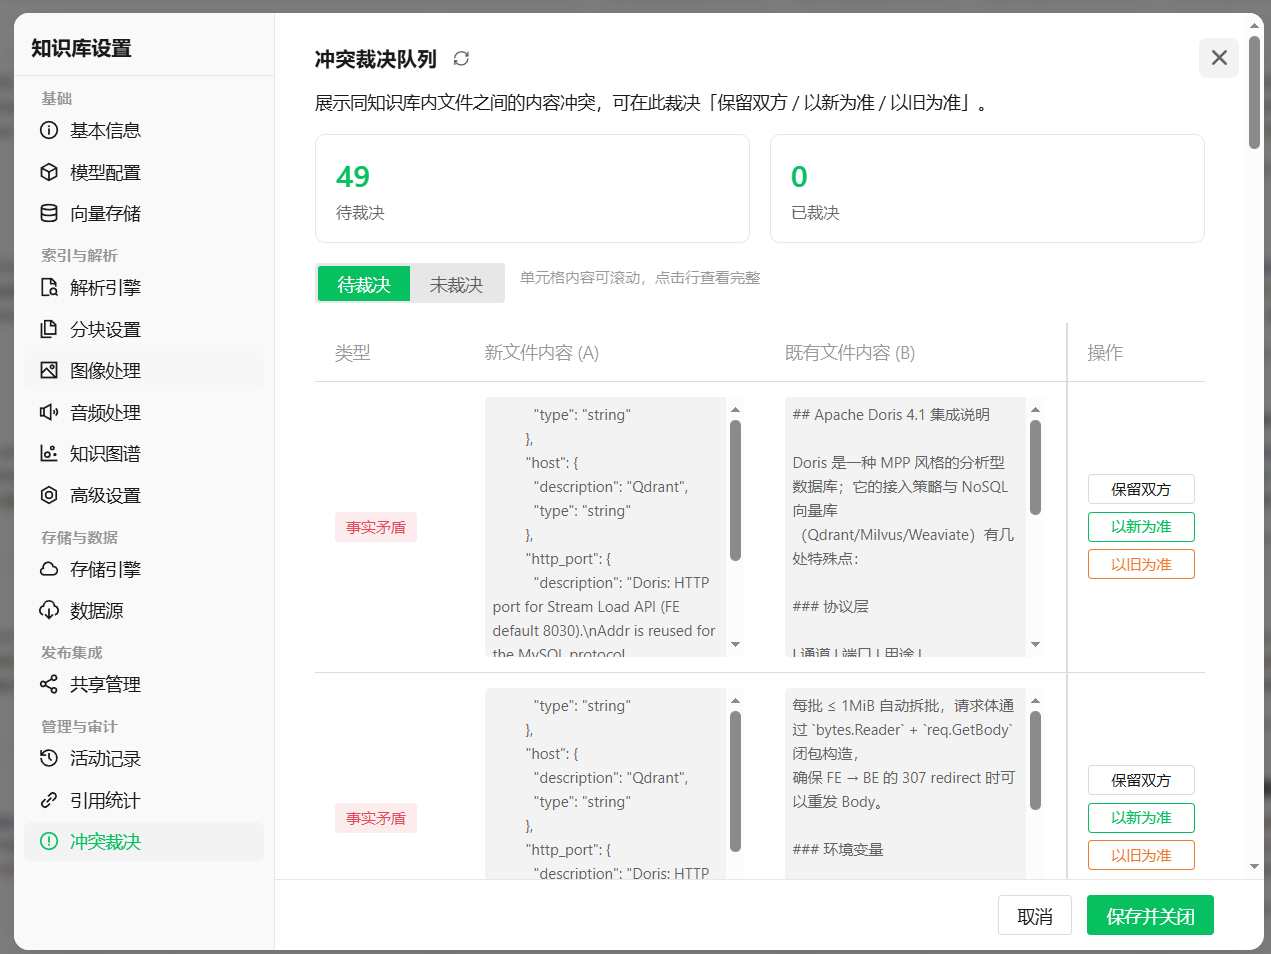
\includegraphics[width=0.45\textwidth]{conflict-queue}}\hfill
  \subfigure[引用计数资产视图]{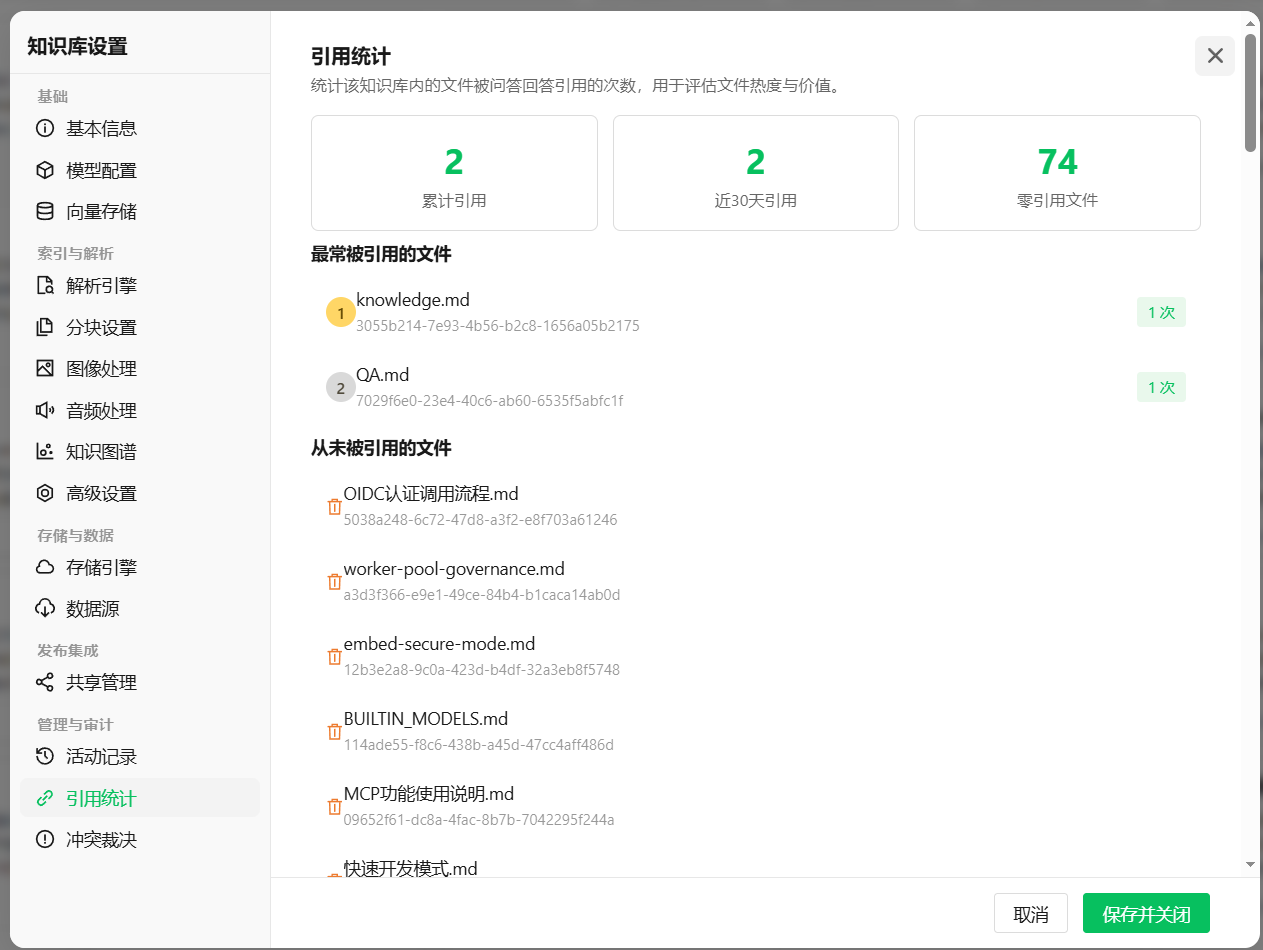
\includegraphics[width=0.45\textwidth]{ref-count}}\\
  \subfigure[文件夹层次治理]{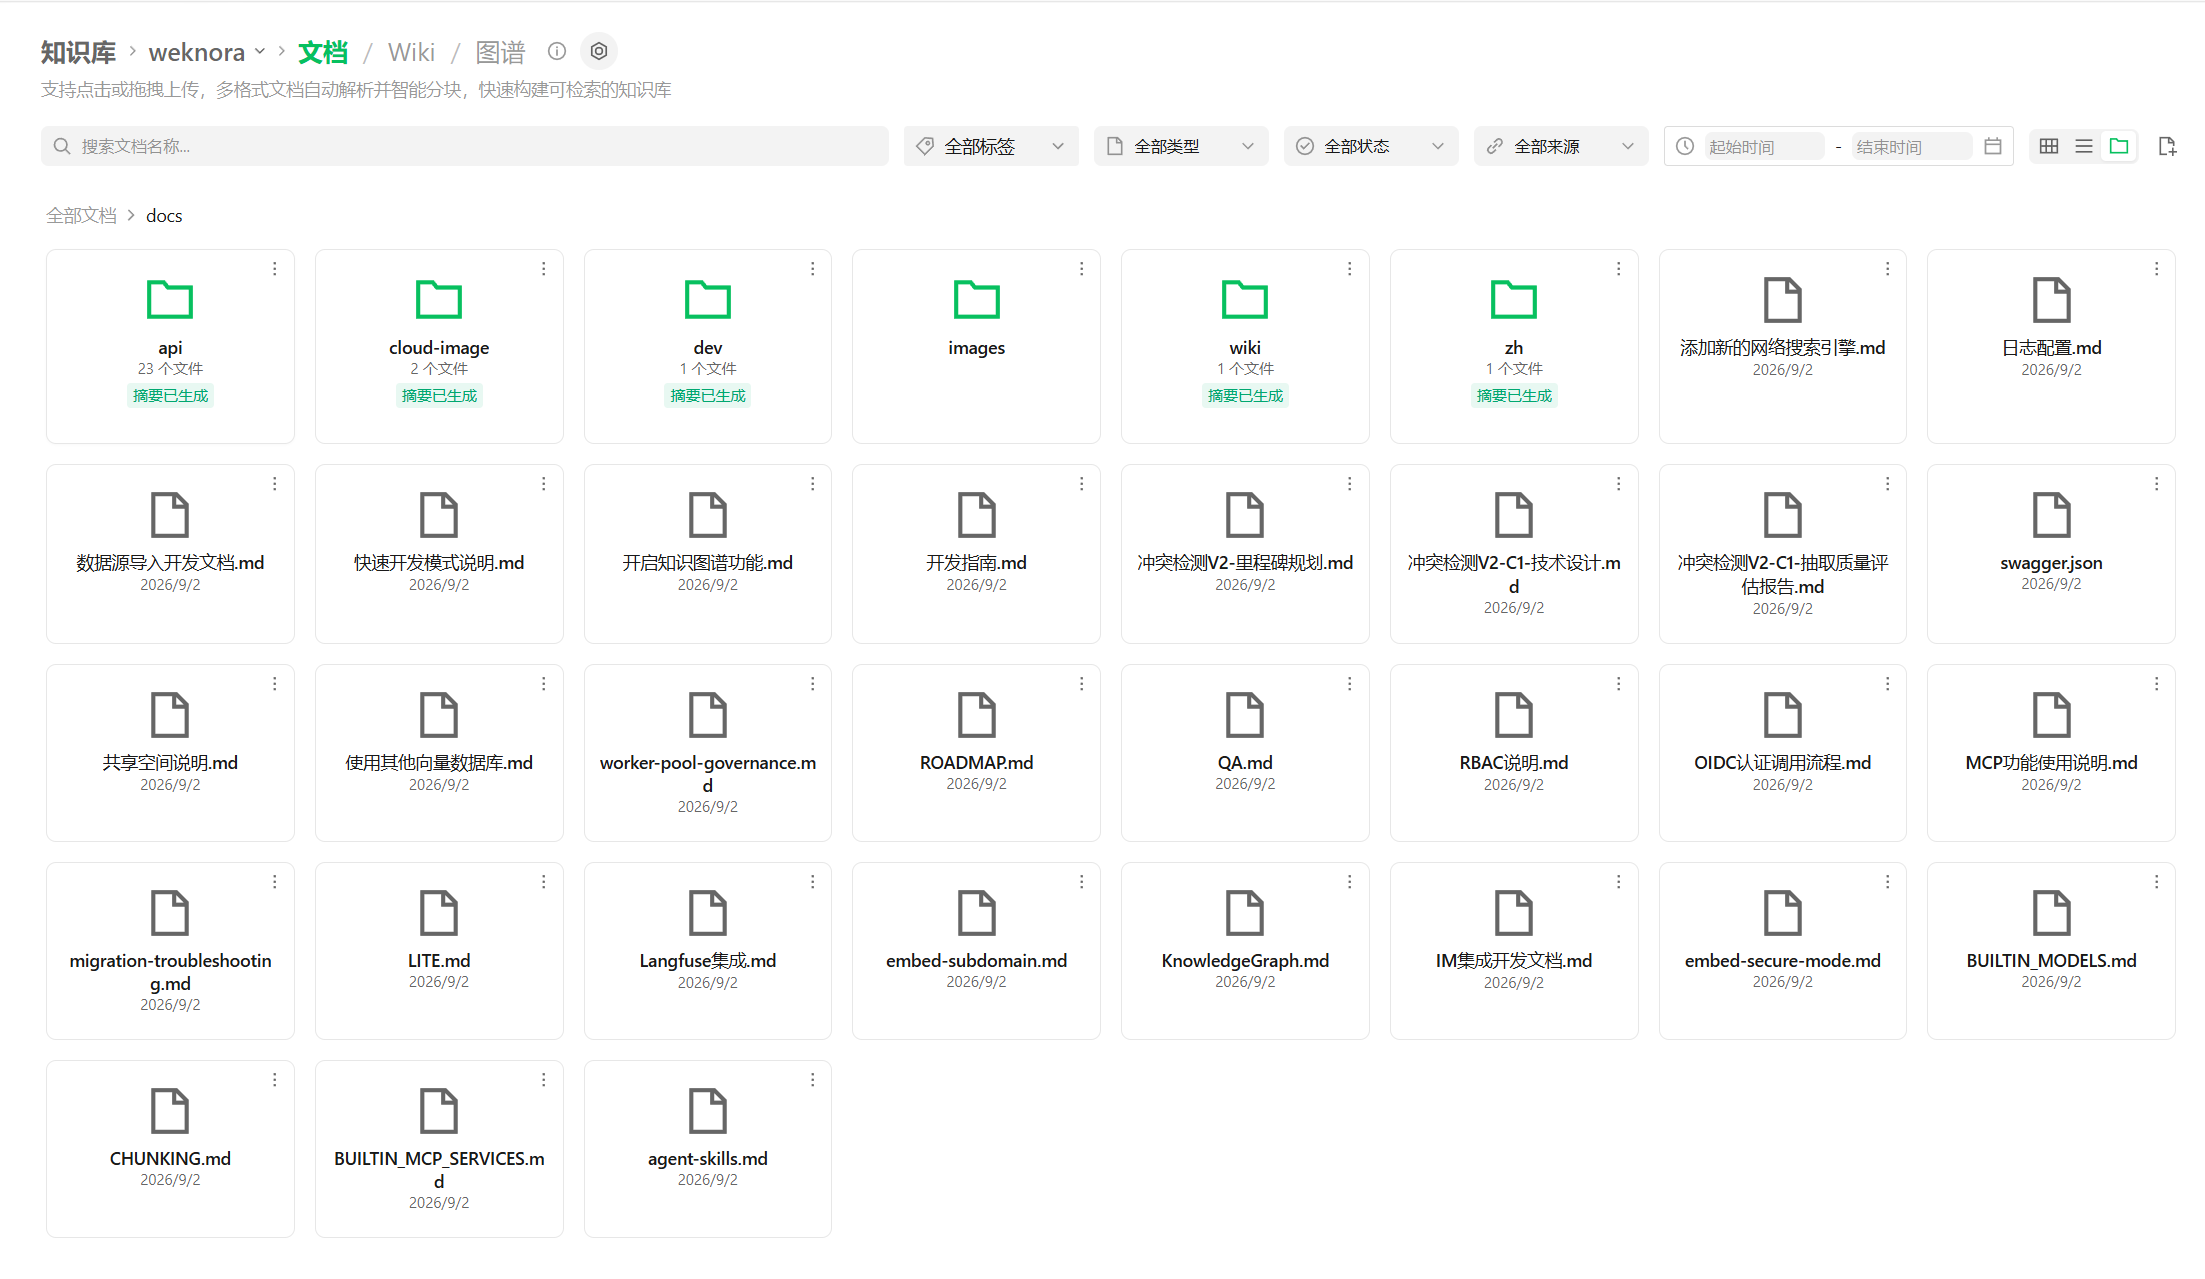
\includegraphics[width=0.45\textwidth]{folder-manage}}\hfill
  \subfigure[反哺 Wiki 审计与回滚]{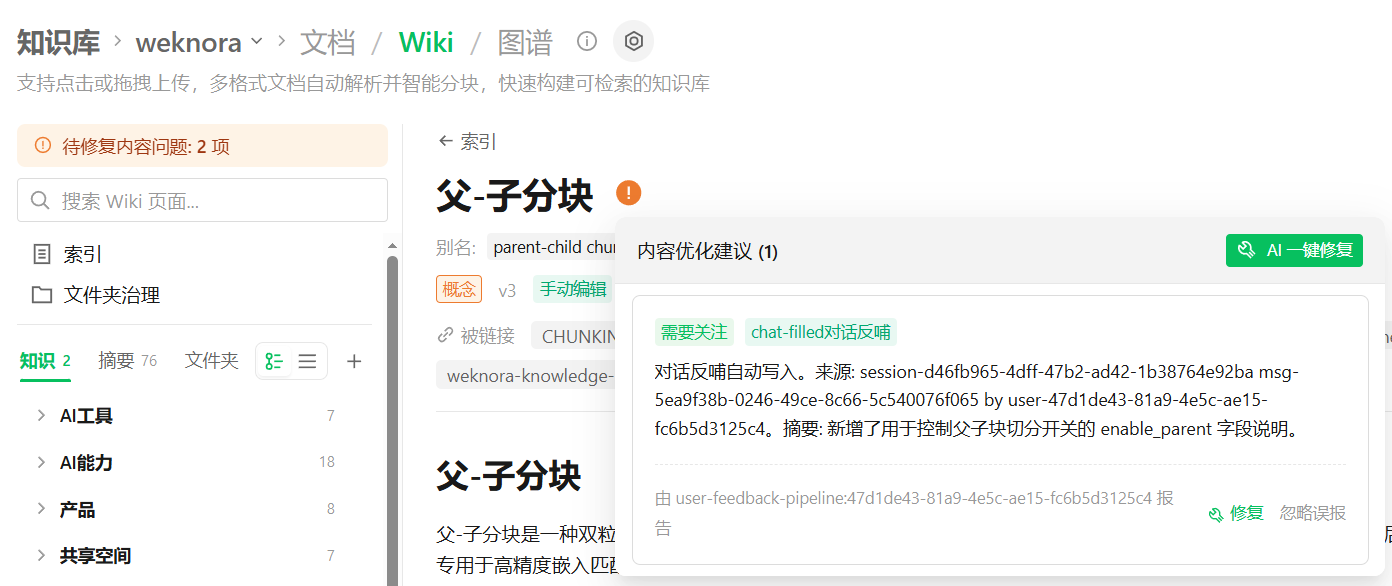
\includegraphics[width=0.45\textwidth]{wiki-report}}
  \caption{前期四项原型工作在 WeKnora 中的界面截图}
  \label{fig:prototype}
\end{figure}

\begin{table}[htbp]
  \centering
  \caption{前期工作与所支撑的研究内容}
  \label{tab:prework}
  \begin{tabular}{p{0.22\textwidth}p{0.44\textwidth}p{0.26\textwidth}}
    \toprule
    前期工作 & 已实现内容 & 支撑的研究内容 \\
    \midrule
    引用计数基础设施 & 引用事件流、多维聚合查询、资产观测视图 & 研究内容二（检索信号）、三（演化评估）、四 \\
    知识冲突检测与消解 & 声明抽取与双通道候选生成、规则与 LLM 级联裁决、争议事实聚合、全局胜方建议与显式采纳、检索冲突惩罚 & 研究内容一（原型）、二 \\
    文件夹层次化治理 & 文件夹树、文件夹摘要防抖生成、范围检索 & 研究内容四 \\
    用户反哺 Wiki 管线 & 全自动异步两阶段写入管线、追加段协议、审计 issue 流、版本快照回滚 & 研究内容三（原型） \\
    \bottomrule
  \end{tabular}
\end{table}

其中，冲突检测管线已在真实服务上完成多轮运行评估：声明级检测在人工标注语料上的查准率与查全率约为 0.87 与 0.84，冲突关键样本召回 15/15；引入确定性规则与灰区批量裁决后，评估场景中冲突判定的 LLM 调用次数由 48 次降至 9 次。这些结果初步验证了声明级级联架构的可行性，也为精度—成本研究提供了基线数据。

\section{学位论文的主要研究内容、实施方案及其可行性论证}

\subsection{主要研究内容}

本课题的研究主线是\textbf{面向内容非一致且持续演化的企业语料，构建可信的检索增强生成能力}。研究内容一治理存量语料中的事实冲突，研究内容二保障冲突证据下的可信生成，研究内容三从对话中吸收增量知识并控制污染，研究内容四提供系统底座并完成端到端验证。总体框架如图~\ref{fig:framework} 所示。

% 图 3：总体研究框架图（AI 生成）
\begin{figure}[htbp]
  \centering
  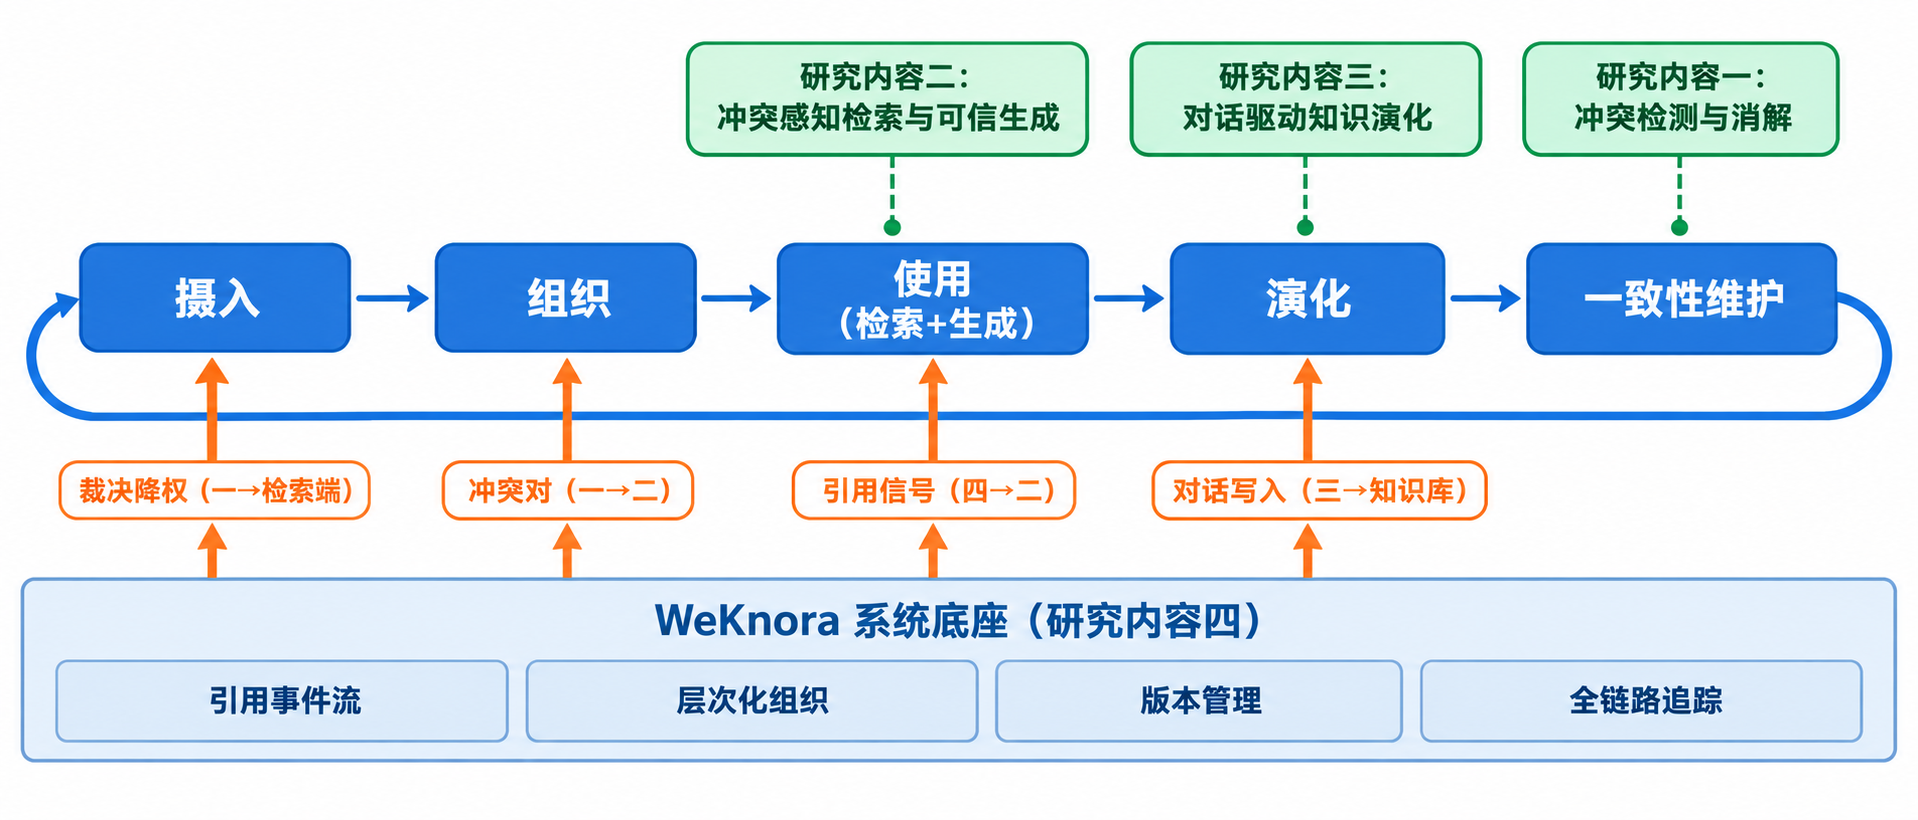
\includegraphics[width=0.95\textwidth]{framework}
  \caption{总体研究框架：沿知识生命周期组织的四个研究内容及其关联}
  \label{fig:framework}
\end{figure}

\subsubsection{研究内容一：多文档知识冲突检测与消解方法}

\textbf{目标}：在成本可控前提下，检测同库跨文档的事实矛盾并支持人机协同消解。

\textbf{具体内容}：
\begin{enumerate}
  \item \textbf{任务形式化}：给定文档集合 $D$ 及其声明集合 $S$（每条声明为由 LLM 抽取的实体—属性—取值三元组，携带来源与时间戳），检测 $S$ 中跨文档的冲突关系并聚合为以事实为单位的争议集合 $F$，每个争议事实汇集全部来源与候选取值，优化目标为检测精度与 LLM 调用成本的联合最优。冲突关系分为四类：\textbf{事实矛盾}指同一实体的同一属性取值互斥；\textbf{局部矛盾}指部分属性互斥、其余信息可共存；\textbf{版本更新}指同一事实取值随时间演替，可由时间戳等元数据佐证；\textbf{非冲突}即互补，表述相近但信息互不矛盾，是检测中最难的负样本；
  \item \textbf{声明级级联检测方法}：先由 LLM 从文档中抽取结构化声明作为比较单元；候选生成采用声明键精确匹配与混合检索回退的双通道，以覆盖同义表述与字段命名漂移；裁决阶段先用确定性规则消解明确情况，同值放行、数值冲突直判，不调用 LLM，仅将灰区候选交由 LLM 批量裁决，并附原文证据约束输出。研究各层级联的通过率、通道分布、批大小与精度—成本曲线的关系；
  \item \textbf{事实级聚合与裁决联动}：将原始冲突记录按稳定的事实锚点聚合为争议事实，同一事实的多来源冲突只呈现一个人工裁决单元；基于版本时间、签发方等元数据给出全局胜方建议，经人工显式采纳后，胜方内容保持检索可用、其余来源禁用退出检索，采纳支持撤销与重开；未决冲突在检索排序阶段施加惩罚因子并保留冲突标记，形成"检测—聚合—裁决—检索"闭环；
  \item \textbf{基准数据集构建}：基于真实文档修订历史与受控扰动合成两条路径构建带标注的企业知识冲突基准，重点构造语义高度相似但互补的干扰对作为高难度负样本。
\end{enumerate}

研究内容一的整体流程如图~\ref{fig:cascade} 所示。

% 图 4：多文档冲突检测与消解全流程（AI 生成；按冲突检测 V2 真实架构的提示词，需重新生成）
\begin{figure}[htbp]
  \centering
  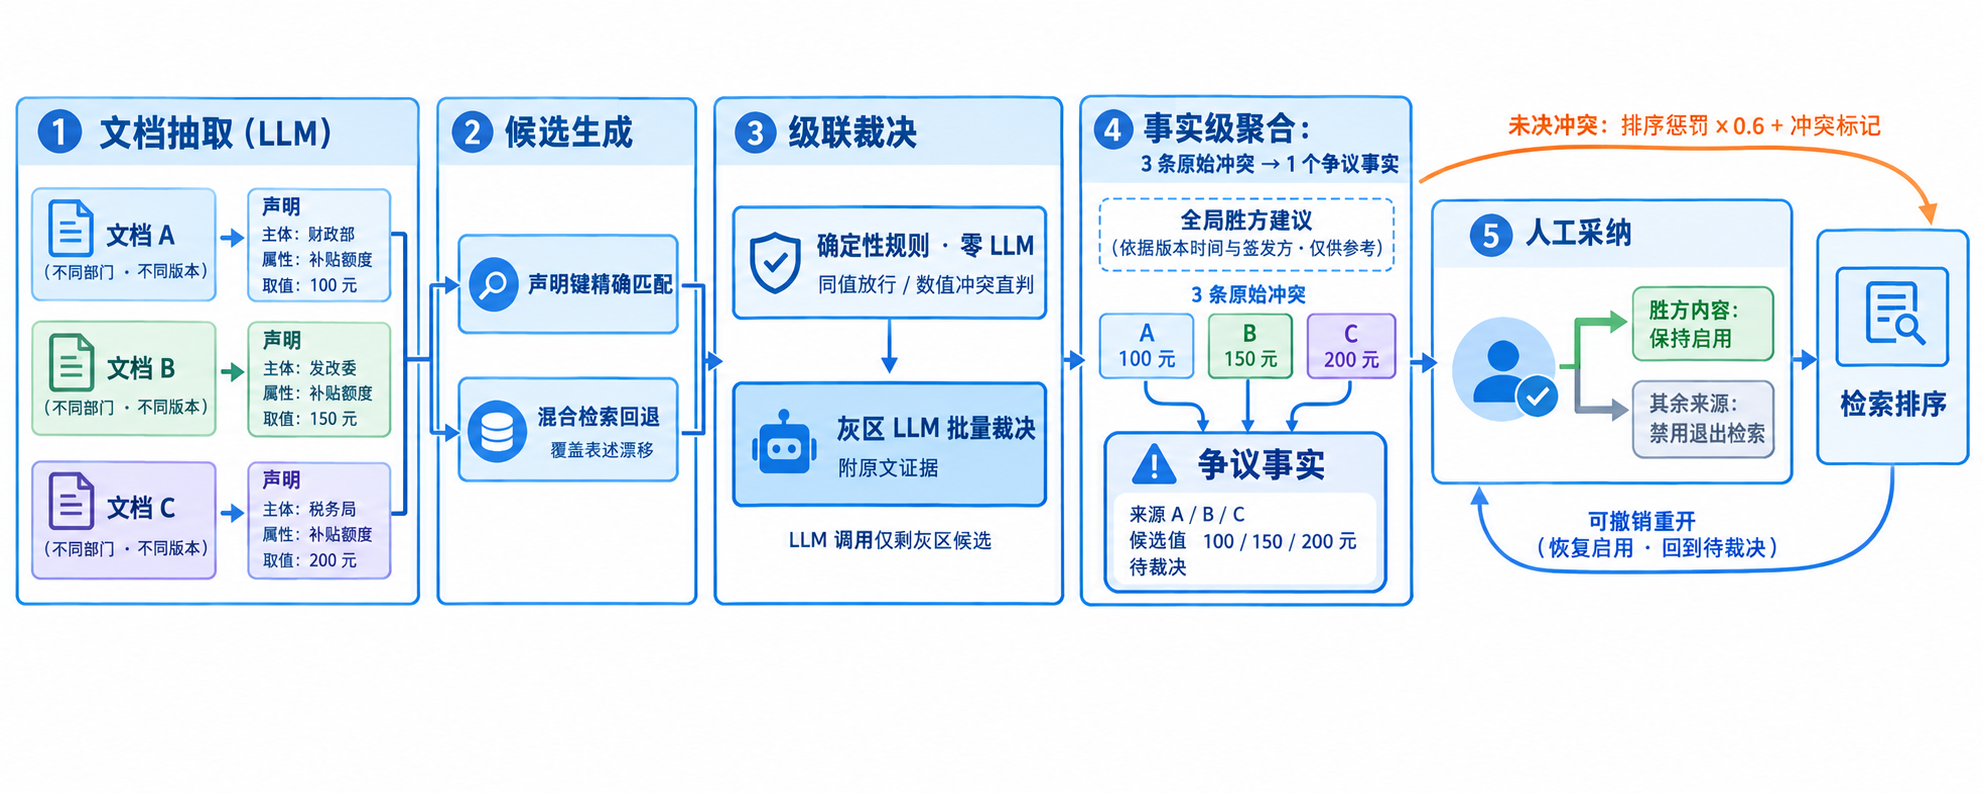
\includegraphics[width=0.98\textwidth]{cascade-pipeline}
  \caption{多文档知识冲突的声明级检测与事实级消解全流程}
  \label{fig:cascade}
\end{figure}

\subsubsection{研究内容二：冲突感知的检索与可信生成方法}

\textbf{目标}：刻画检索证据内部存在矛盾时 LLM 的生成行为，并提出缓解方法。

\textbf{具体内容}：
\begin{enumerate}
  \item \textbf{行为刻画}：基于研究内容一构建的冲突对构造"命中矛盾证据"的问答集，对多个主流 LLM 在标准 RAG 管线下的回答进行行为分类，划分为正确呈现分歧、盲从一方、幻觉调和、拒答等类别，并分析长上下文中位置带来的证据顺序偏差 \cite{liu2024}、来源标注、时间戳提示等因素的影响；
  \item \textbf{冲突感知检索}：将工程原型中的冲突降权启发式升级为\textbf{可信度感知排序}：融合来源时效性、冲突状态与历史引用信号（研究内容四）的多维可信度模型，研究其对检索质量与下游回答的影响；
  \item \textbf{冲突感知生成策略}：以对比方式呈现矛盾双方及其来源与时间戳，信息不可判定时拒答，与降权策略组合评测；
  \item \textbf{评测协议}：建立冲突场景下生成质量的自动评测与人工评测子集，其中自动评测采用 LLM-as-judge 并辅以人工校准，报告一致性系数。
\end{enumerate}

矛盾证据下生成行为的分类示例如图~\ref{fig:behavior} 所示。

% 图 5：矛盾证据下的生成行为分类示例（AI 生成）
\begin{figure}[htbp]
  \centering
  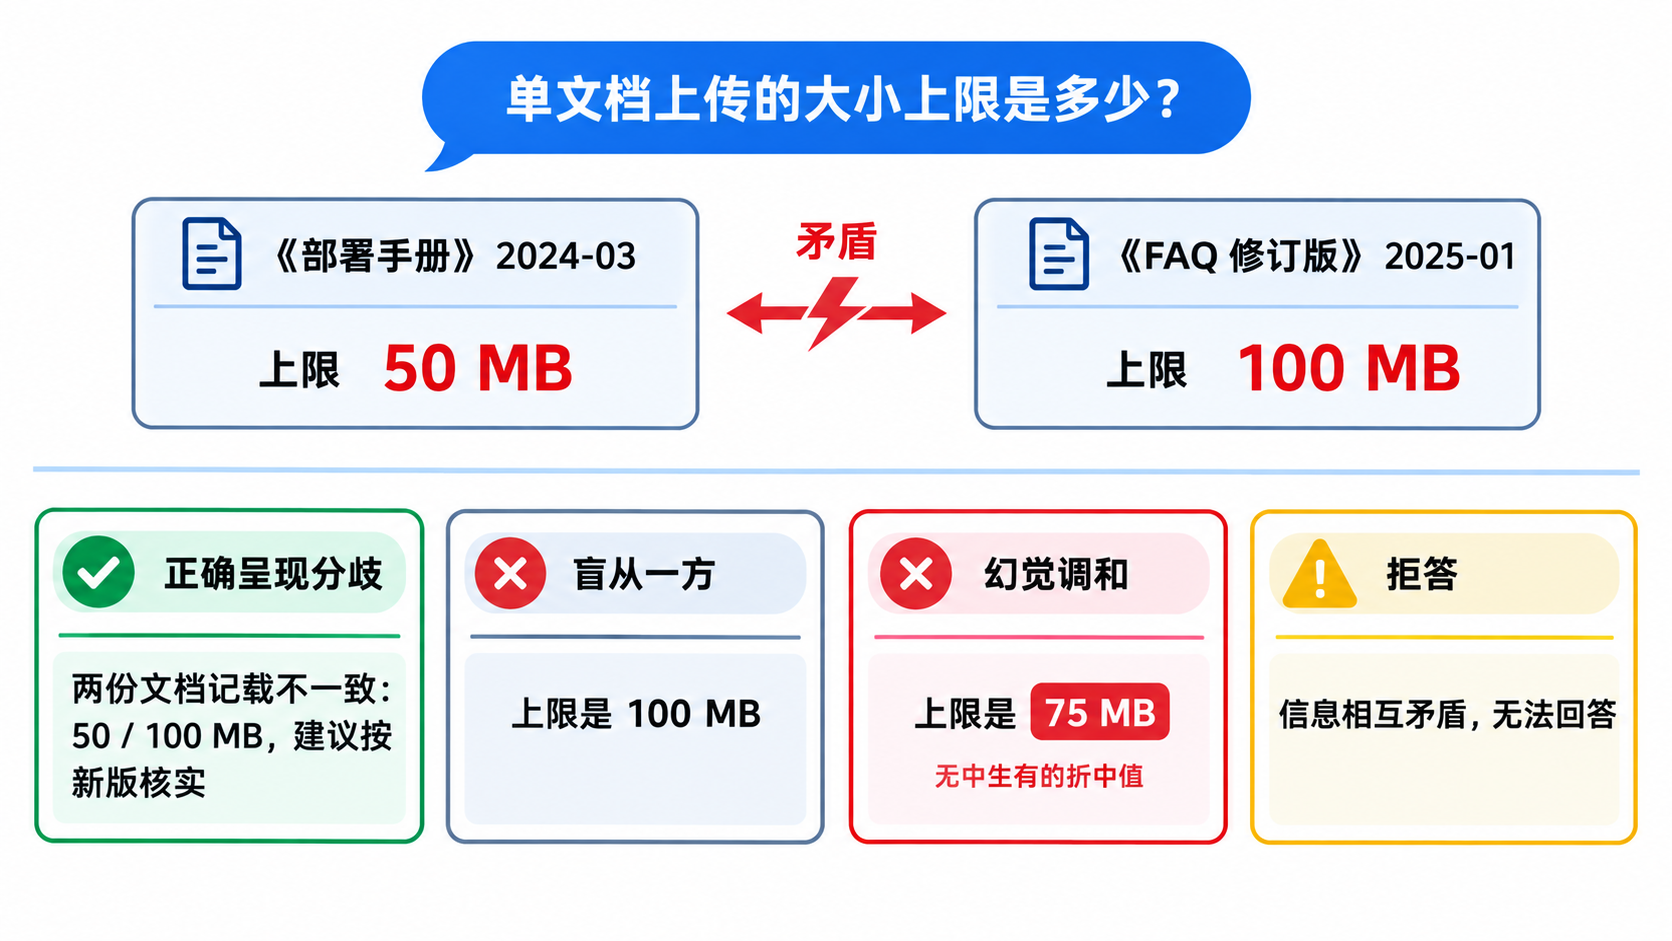
\includegraphics[width=0.85\textwidth]{behavior-taxonomy}
  \caption{检索证据内部矛盾下的 LLM 生成行为分类（示例）}
  \label{fig:behavior}
\end{figure}

\subsubsection{研究内容三：对话驱动的知识库持续演化方法}

\textbf{目标}：从用户对话中吸收增量知识入库，同时控制噪声污染风险。

\textbf{具体内容}：
\begin{enumerate}
  \item \textbf{知识写入决策问题定义}：形式化为三段决策——是否写入（用户消息是否包含值得沉淀的新事实）、写到何处（应写入知识库的哪个位置）、如何写入（增量合并且不破坏原文）；
  \item \textbf{两阶段写入管线}：第一阶段轻量判断消息有效性，区分陈述事实与提问、闲聊、观点；第二阶段检索候选页面并规划追加内容；研究两阶段的模型规模分配与成本优化；
  \item \textbf{审计与回滚机制}：所有自动写入附带版本快照与审计标记，支持事后人工复核、回滚与裁决；
  \item \textbf{模拟演化环境与评测协议}：构建"种子知识库 + 已知 ground truth 的模拟用户消息流 + 时序回放"的演化环境，定义沉淀率（写入精度、位置准确率、内容忠实度）、下游净增益（反哺后问答正确率提升）、污染率（错误信息入库比例及传染性）、演化曲线（多轮后知识库质量收敛/劣化）四类指标。
\end{enumerate}

图~\ref{fig:pipeline} 给出写入管线与三重风险防线的设计。

% 图 6：两阶段写入管线与三重防线（AI 生成）
\begin{figure}[htbp]
  \centering
  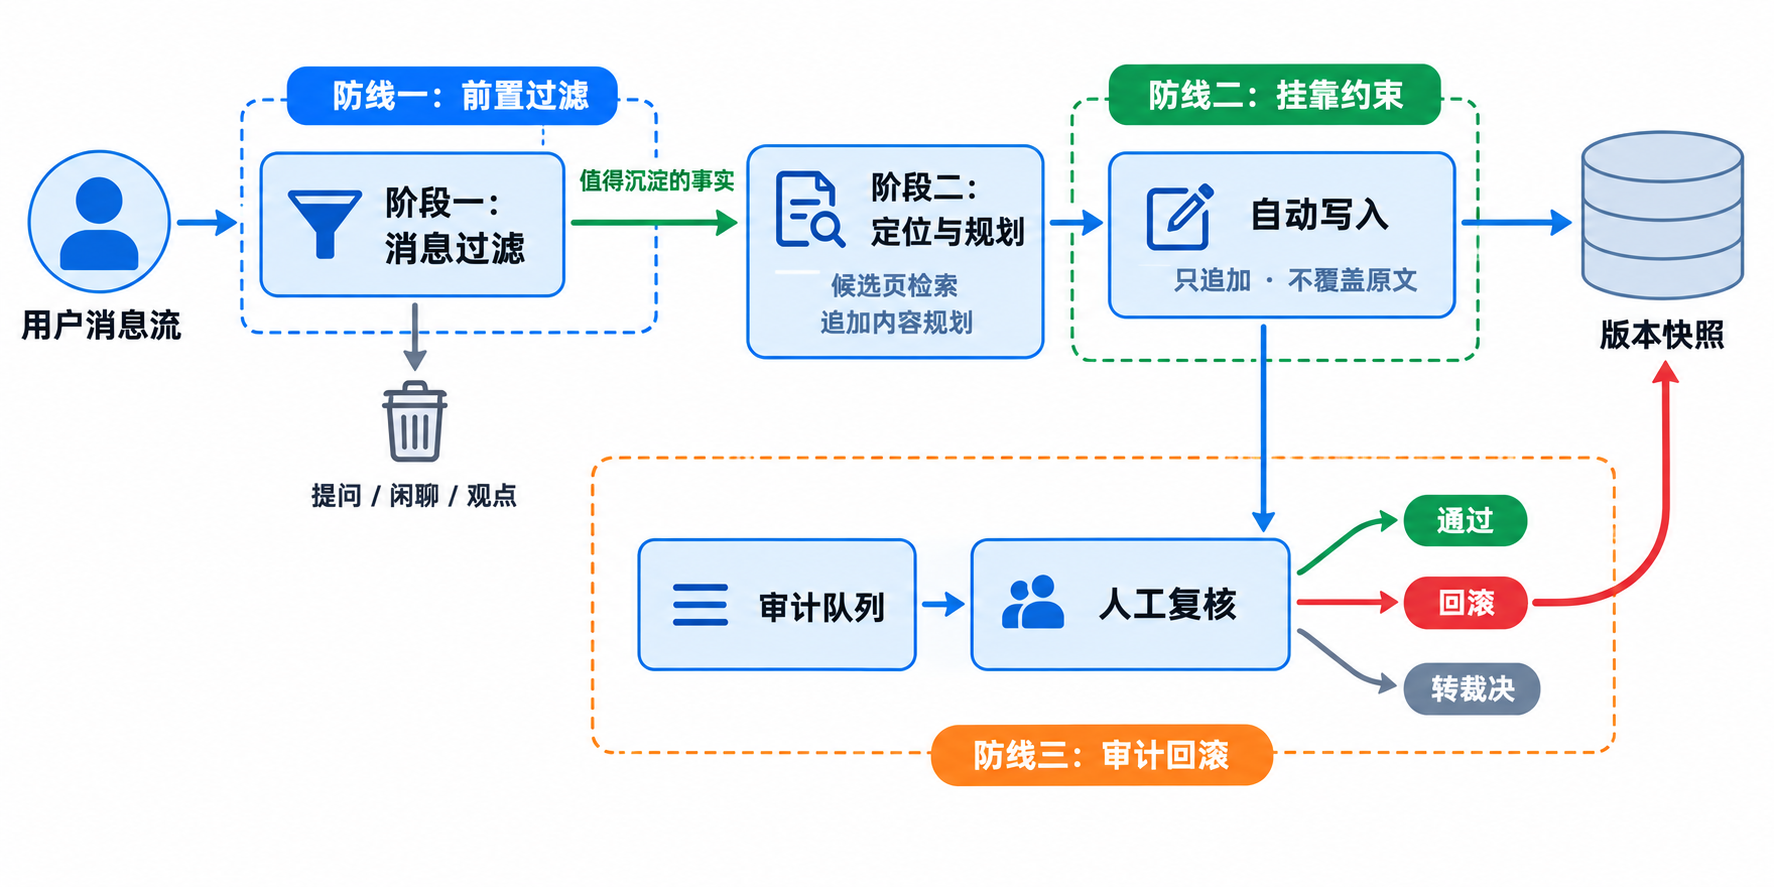
\includegraphics[width=0.92\textwidth]{write-pipeline}
  \caption{对话驱动的知识写入管线及其风险控制防线}
  \label{fig:pipeline}
\end{figure}

\subsubsection{研究内容四：面向知识生命周期的系统实现与端到端验证}

\textbf{目标}：在真实系统上完成从摄入、组织、使用到演化与一致性维护的全流程实现与验证。

\textbf{具体内容}：
\begin{enumerate}
  \item \textbf{知识使用信号观测}：以回答实际引用而非检索召回为准建立引用事件流，支持文件级、库级与时间窗口聚合，为研究内容二的检索加权与研究内容三的演化质量评估提供信号；
  \item \textbf{层次化知识组织与生命周期管理}：采用邻接表与物化路径组织文件级文件夹树，通过防抖生成、级联刷新实现文件夹摘要的增量维护，支持范围检索与子域背景注入，并处理上传替换时引用事件与冲突记录的级联清理；
  \item \textbf{端到端集成与真实环境评估}：全部能力在开源框架 WeKnora 上以"按库渐进开启"的增量方式集成，结合全链路追踪系统采集真实运行数据，如裁决队列中的人工纠错比例，作为方法评估的补充证据。
\end{enumerate}

\subsection{实施方案及其可行性论证}

\subsubsection{总体方案}

依托 WeKnora 开源框架搭建实验平台，前期四项原型工作（见表~\ref{tab:prework}）已打通从摄入、组织、使用到演化的核心链路，本课题在此基础上按研究内容逐项开展方法研究与实验验证。优先级上，研究内容一、二构成方法主线，研究内容三紧随其后，研究内容四以工程增量方式伴随全程，不单独占用实验周期。

\subsubsection{研究内容一的实验设计}

\begin{itemize}
  \item \textbf{数据集}：\textcircled{1} 真实修订历史——采集真实企业内部文档/产品手册的多版本文件，标注版本更新与跨版本矛盾；\textcircled{2} 受控合成——将种子事实句经 LLM 改写数值、否定或时间等受控扰动后注入文档，构造已知 ground truth 的冲突，重点构造"高相似但互补"的困难负样本；\textcircled{3} 真实语料人工标注测试集——对真实多版本文档语料双人独立标注并仲裁分歧，检验方法在真实分布上的表现；
  \item \textbf{基线}：chunk 相似度候选加逐对 LLM 精判（关闭声明抽取的退化形态）；embedding 相似度阈值直判（验证"相似$\neq$矛盾"）；句对 NLI 模型如 DeBERTa 系（验证传统 NLI 在版本更新类上的局限）；LLM 全量两两精判（验证级联的成本优势）；声明级级联方法；
  \item \textbf{指标}：冲突发现 P/R/F1（声明级与事实级），构造全集已知的测试集上直接计算、真实语料上以人工抽检估计召回；冲突类型分类准确率；LLM 调用次数与 token 成本，通过精度—成本 Pareto 曲线呈现；端到端时延；
  \item \textbf{消融与分析}：候选通道消融（仅声明键精确匹配、仅混合检索回退、双通道）、去规则层（全部交由 LLM）、批量裁决批大小扫描、声明抽取开关、去时间戳元数据；冲突类型混淆矩阵与按跨主题、同主题同实体等难度分层的性能对比；辅以真实系统裁决队列的人工纠错比例评估实际效果。
\end{itemize}

\subsubsection{研究内容二的实验设计}

\begin{itemize}
  \item \textbf{数据}：基于研究内容一的冲突对构造 QA 集，确保每个问题命中矛盾证据对；
  \item \textbf{对比条件}：标准 RAG（矛盾证据全量入上下文）/ 冲突降权检索 / 冲突感知提示词 / 结构化对比呈现（本方法）/ 干净知识库 oracle 上界；
  \item \textbf{被测模型}：不少于 3 个主流 LLM，例如 GPT、Qwen、DeepSeek 等系列；
  \item \textbf{指标}：正确呈现分歧、盲从、幻觉调和、拒答等行为分类分布及其正确性，LLM-as-judge 忠实性评分，证据顺序敏感性分析；
  \item \textbf{消融}：降权因子扫描、有无时间戳提示、有无来源标注。
\end{itemize}

\subsubsection{研究内容三的实验设计}

\begin{itemize}
  \item \textbf{模拟演化环境}：由种子知识库、LLM 生成的模拟用户消息流与多轮时序回放构成，消息流中既含应写入的正例，也混入提问、闲聊、观点、已知信息等不应写入的干扰；
  \item \textbf{基线}：不反哺 / 无第一阶段过滤的全量写入 / Mem0 式记忆管理直接迁移 / 逐一确认的显式确认模式；
  \item \textbf{指标}：写入决策 P/R、位置准确率、写入内容忠实度、\textbf{下游 QA 净增益}、污染率及其在后续多轮对话中的传染、多轮演化质量曲线、每条消息成本；
  \item \textbf{消融}：第一阶段模型规模、有无已知信息去重、审计回滚对污染的抑制效果。
\end{itemize}

\subsubsection{研究内容四的验证方案}

\begin{itemize}
  \item 参照前期里程碑的验收标准体系开展端到端功能验证；
  \item 真实运行数据采集与分析：全链路追踪下的引用分布、冲突检测误报的人工纠正率、反哺内容被后续引用与回滚情况的统计；
  \item 系统开销评估：各能力的额外计算成本与延迟影响。
\end{itemize}

\subsubsection{关键技术与难点}

\begin{enumerate}
  \item \textbf{冲突判定精度}（难点）：语义相似与事实矛盾的区分依赖精判模型能力，拟通过冲突分类体系设计、元数据辅助、难度分层负样本与提示策略优化缓解；
  \item \textbf{写入决策的噪声控制}（难点）：全自动写入的污染风险，拟通过两阶段过滤、只追加不覆盖的写入约束与事后审计回滚加以控制；
  \item \textbf{评测的可信性}（方法论难点）：LLM-as-judge 的偏差，拟通过人工校准子集、多 judge 交叉、一致性系数报告控制；
  \item \textbf{成本约束}：企业场景对 LLM 开销敏感，级联架构与小模型分工是贯穿性优化手段。
\end{enumerate}

\subsubsection{可行性分析}

\begin{enumerate}
  \item \textbf{平台可行性}：依托开源框架 WeKnora，引用计数、冲突检测、层次治理、用户反哺四项核心能力已有可运行原型，工程基础扎实，实验可快速开展；
  \item \textbf{技术可行性}：声明抽取与候选生成所需的 LLM 与向量检索、批量裁决与评测所需的任务队列和追踪体系均已在原型中打通；
  \item \textbf{数据可行性}：冲突基准的修订历史采集与受控合成两条构建路径均已验证可操作；模拟演化环境不依赖真实用户隐私数据。
\end{enumerate}

\section{论文进度安排，预期达到的目标}

\subsection{进度安排}

按 2026 年 9 月起约 15 个月，结题答辩定于 2027 年 12 月：

\begin{table}[htbp]
  \centering
  \caption{研究进度安排}
  \label{tab:schedule}
  \begin{tabular}{cp{0.20\textwidth}p{0.62\textwidth}}
    \toprule
    阶段 & 时间 & 工作内容 \\
    \midrule
    1 & 2026.09--2026.10 & 文献精读与查新；冲突检测基准数据集构建（修订历史采集 + 受控合成）；完成开题 \\
    2 & 2026.10--2027.01 & 研究内容一：声明级级联检测实验、基线对比与消融；撰写小论文\textcircled{1} \\
    3 & 2027.01--2027.03 & 研究内容二：冲突 QA 构造、行为刻画与生成策略实验；小论文\textcircled{1}投稿；撰写小论文\textcircled{2} \\
    4 & 2027.03--2027.05 & 研究内容三：模拟演化环境、反哺管线实验；小论文\textcircled{2}投稿；中期答辩 \\
    5 & 2027.05--2027.07 & 研究内容四：系统端到端集成与真实环境评估；整理开源成果 \\
    6 & 2027.07--2027.10 & 学位论文撰写 \\
    7 & 2027.10--2027.12 & 论文修改、预答辩、结题答辩 \\
    \bottomrule
  \end{tabular}
\end{table}


\subsection{预期达到的目标}

\begin{table}[htbp]
  \centering
  \caption{预期成果}
  \label{tab:achieve}
  \begin{tabular}{p{0.16\textwidth}p{0.76\textwidth}}
    \toprule
    类型 & 预期成果 \\
    \midrule
    学术论文 & 在 CCF-B/C 类国际会议投稿论文 1--2 篇，力争答辩前录用 1 篇 \\
    数据与基准 & 企业知识冲突检测基准数据集 1 套（含评测脚本）；知识库演化模拟评测环境 1 套 \\
    系统成果 & 上述能力在开源框架上的完整实现（开源贡献） \\
    学位论文 & 完成硕士学位论文 1 部 \\
    \bottomrule
  \end{tabular}
\end{table}

\section{学位论文预期创新点}

\begin{enumerate}
  \item \textbf{任务与基准创新}：将企业知识库的多文档事实冲突检测形式化为语料级冲突对发现问题，构建面向企业场景、含版本更新特殊类别的冲突检测基准数据集，与面向维基百科、定位生成端评测的现有基准形成互补；
  \item \textbf{方法创新}：提出"声明级级联检测—事实级聚合—裁决联动检索"的冲突治理闭环，以确定性规则与灰区批量 LLM 裁决控制成本，将多来源冲突聚合为单一争议事实支撑人机协同裁决；
  \item \textbf{发现与方法创新}：分析大模型在检索证据内部矛盾下的生成行为（含“幻觉调和”等现象的刻画），提出冲突感知的可信度排序与对比式生成策略；
  \item \textbf{问题定义与协议创新}：提出知识写入决策问题及沉淀与污染权衡的评测协议，实现带审计回滚的对话驱动知识库演化。
\end{enumerate}

\section{为完成课题已具备和所需的条件、外协计划及经费}

\textbf{已具备的条件}：
\begin{enumerate}
  \item 依托 WeKnora 开源框架及引用计数、冲突检测、层次治理、用户反哺四项可运行原型，具备完整的实验平台；
  \item 具备 GPT、Qwen、DeepSeek 等主流 LLM API 的调用能力，以及向量检索、全链路追踪等基础设施；
  \item 企业已有大量真实文档与产品手册等语料资源，可作为基准数据集构建的素材来源。
\end{enumerate}

\textbf{所需条件与外协计划}：本课题以开源框架与公共 LLM API 为主要实验手段，计算资源主要用于评测集构建与 NLI 基线微调，其中 GPU 算力拟使用实验室现有服务器；不涉及需外协完成的定制实验设备或数据采购。

\textbf{经费预算}：主要开销为用于评测与合成数据生成的 LLM API 调用费用，以及算力租用，预算规模视评测规模而定，拟通过实验室科研经费列支。

\section{预计研究过程中可能遇到的困难、问题，以及解决的途径}

\begin{enumerate}
  \item \textbf{冲突判定精度受限于精判模型能力}：语义相似与事实矛盾在表述层面高度接近，现有 LLM 精判存在系统性偏差。解决途径：设计细粒度冲突分类体系、引入文档时间戳等元数据辅助、构造难度分层的负样本并优化提示策略；
  \item \textbf{全自动知识沉淀的污染风险}：错误写入的知识可能随检索传播放大。解决途径：两阶段过滤前置拦截、只追加不覆盖原文的写入约束，配合事后审计与回滚，并在评测协议中将污染率及其传染性作为核心指标度量，同时完整记录污染的发生条件与传播路径，为权衡分析提供实证材料；
  \item \textbf{LLM-as-judge 评测偏差}：自动评测的可信性存疑。解决途径：设置人工校准子集、多 judge 交叉投票，并报告与人工标注的一致性系数，以 $\geq 0.7$ 为目标；
  \item \textbf{成本约束}：企业场景对 LLM 开销敏感，全量两两精判成本不可接受。解决途径：以确定性规则先行、灰区批量 LLM 裁决的级联架构与小模型分工作为贯穿性优化手段，以精度—成本 Pareto 曲线为考核指标。
\end{enumerate}

\section{主要参考文献}

\bibliographystyle{hithesis}
\bibliography{reference}
% 新增文献条目（hou2024wikicontradict / chhablani2025 / yin2008 / li2015 / liu2024）
% 已并入本目录 reference.bib。

% Local Variables:
% TeX-master: "../report"
% TeX-engine: xetex
% End:


% 威海校区本科生开题报告结构 ----------------------------------------
% % !Mode:: "TeX:UTF-8"
\section{课题背景及研究的目的和意义}
\subsection{课题背景}
（正文  宋体小4号字，多倍行距值1.25，段前0行，段后0行。字数3000字以上。具体的撰写要符合哈尔滨工业大学本科生毕业论文撰写规范的书写规定。）\cite{hithesis2017}\inlinecite{cnproceed}
\subsection{研究的目的和意义}
\section{国内外在该方向的研究现状及分析}
\subsection{国外现状及分析}
\subsection{国内现状及分析}
\section{研究内容及拟解决的关键问题}
\subsection{研究内容}
\subsection{拟解决的关键问题}
\section{拟采取的研究方法和技术路线、进度安排、预期达到的目标}
\subsection{拟采取的研究方法和技术路线}
\subsection{进度安排}
\subsection{预期达到的目标}
\section{课题已具备和所需的条件}
\section{研究过程中可能遇到的困难和问题，解决的措施}
\section{参考文献}
\bibliographystyle{hithesis}
\bibliography{reference}

% Local Variables:
% TeX-master: "../report"
% TeX-engine: xetex
% End:
% \makebackcover
% -------------------------------------------------------------

% 威海校区本科生中期报告结构 ----------------------------------------
% \section{论文工作是否按预期进行、目前已完成的研究工作及结果}
\subsection{论文工作是否按预期进行}
（正文  宋体小4号字，多倍行距值1.25，段前0行，段后0行。字数3000字以上。具体的撰写要符合哈尔滨工业大学本科生毕业论文撰写规范的书写规定。）
\subsection{目前已完成的研究工作及结果}
\section{后期拟完成的研究工作及进度安排}
\subsection{后期拟完成的研究工作}
\subsection{后期进度安排}
\section{存在的问题与困难}
\section{论文按时完成的可能性}
\section{参考文献}
\bibliographystyle{hithesis}
\bibliography{reference}

% Local Variables:
% TeX-master: "../mainart"
% TeX-engine: xetex
% End:
% \makebackcover
% -------------------------------------------------------------

% 哈尔滨校区本科生开题报告结构 --------------------------------------
% \section{课题来源及研究的目	的和意义}
（正文  宋体小4号字，行距1.25倍，段前0行，段后0行）
\section{国内外在该方向的研究现状及分析}
\section{主要研究内容}
\section{研究方案}
\section{进度安排，预期达到的目标}
\section{课题已具备和所需的条件、经费}
\section{研究过程中可能遇到的困难和问题，解决的措施}
\section{主要参考文献}
\bibliographystyle{hithesis}
\bibliography{reference}

% Local Variables:
% TeX-master: "../mainart"
% TeX-engine: xetex
% End:
% -------------------------------------------------------------

\end{document}

% Local Variables:
% TeX-engine: xetex
% End:
